\pagebreak
\clearpage
\section{Supplementary Material}
\label{sec:sm}
 In this section we show the results of some extended tests.
 section~\ref{subsec:glass} shows our results on glass fibers. Section~\ref{subsec:vox_ex} shows the some more results of voxelization and mesh generation. Section~\ref{subsec:compare} shows comparisons to hierarchical clustering and with individual fiber extraction technique. Finally, section~\ref{subsec:robustness} shows another result with different parameter to show robustness of parameter selection.
 
\begin{figure}
\centering
\subfloat[]{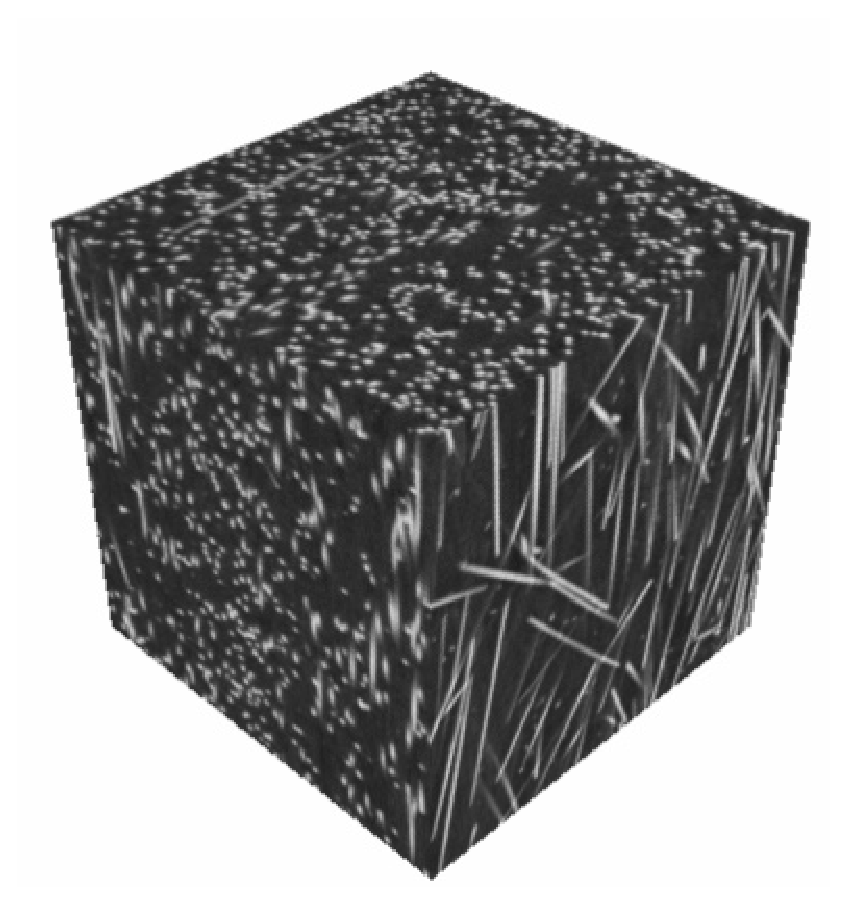
\includegraphics[width=0.25\linewidth]{imagesMT2014/glass-scalar.eps}}
  \subfloat[]{
\includegraphics[width=0.25\linewidth]{imagesMT2014/glass-scalar-slice}}
  \subfloat[]{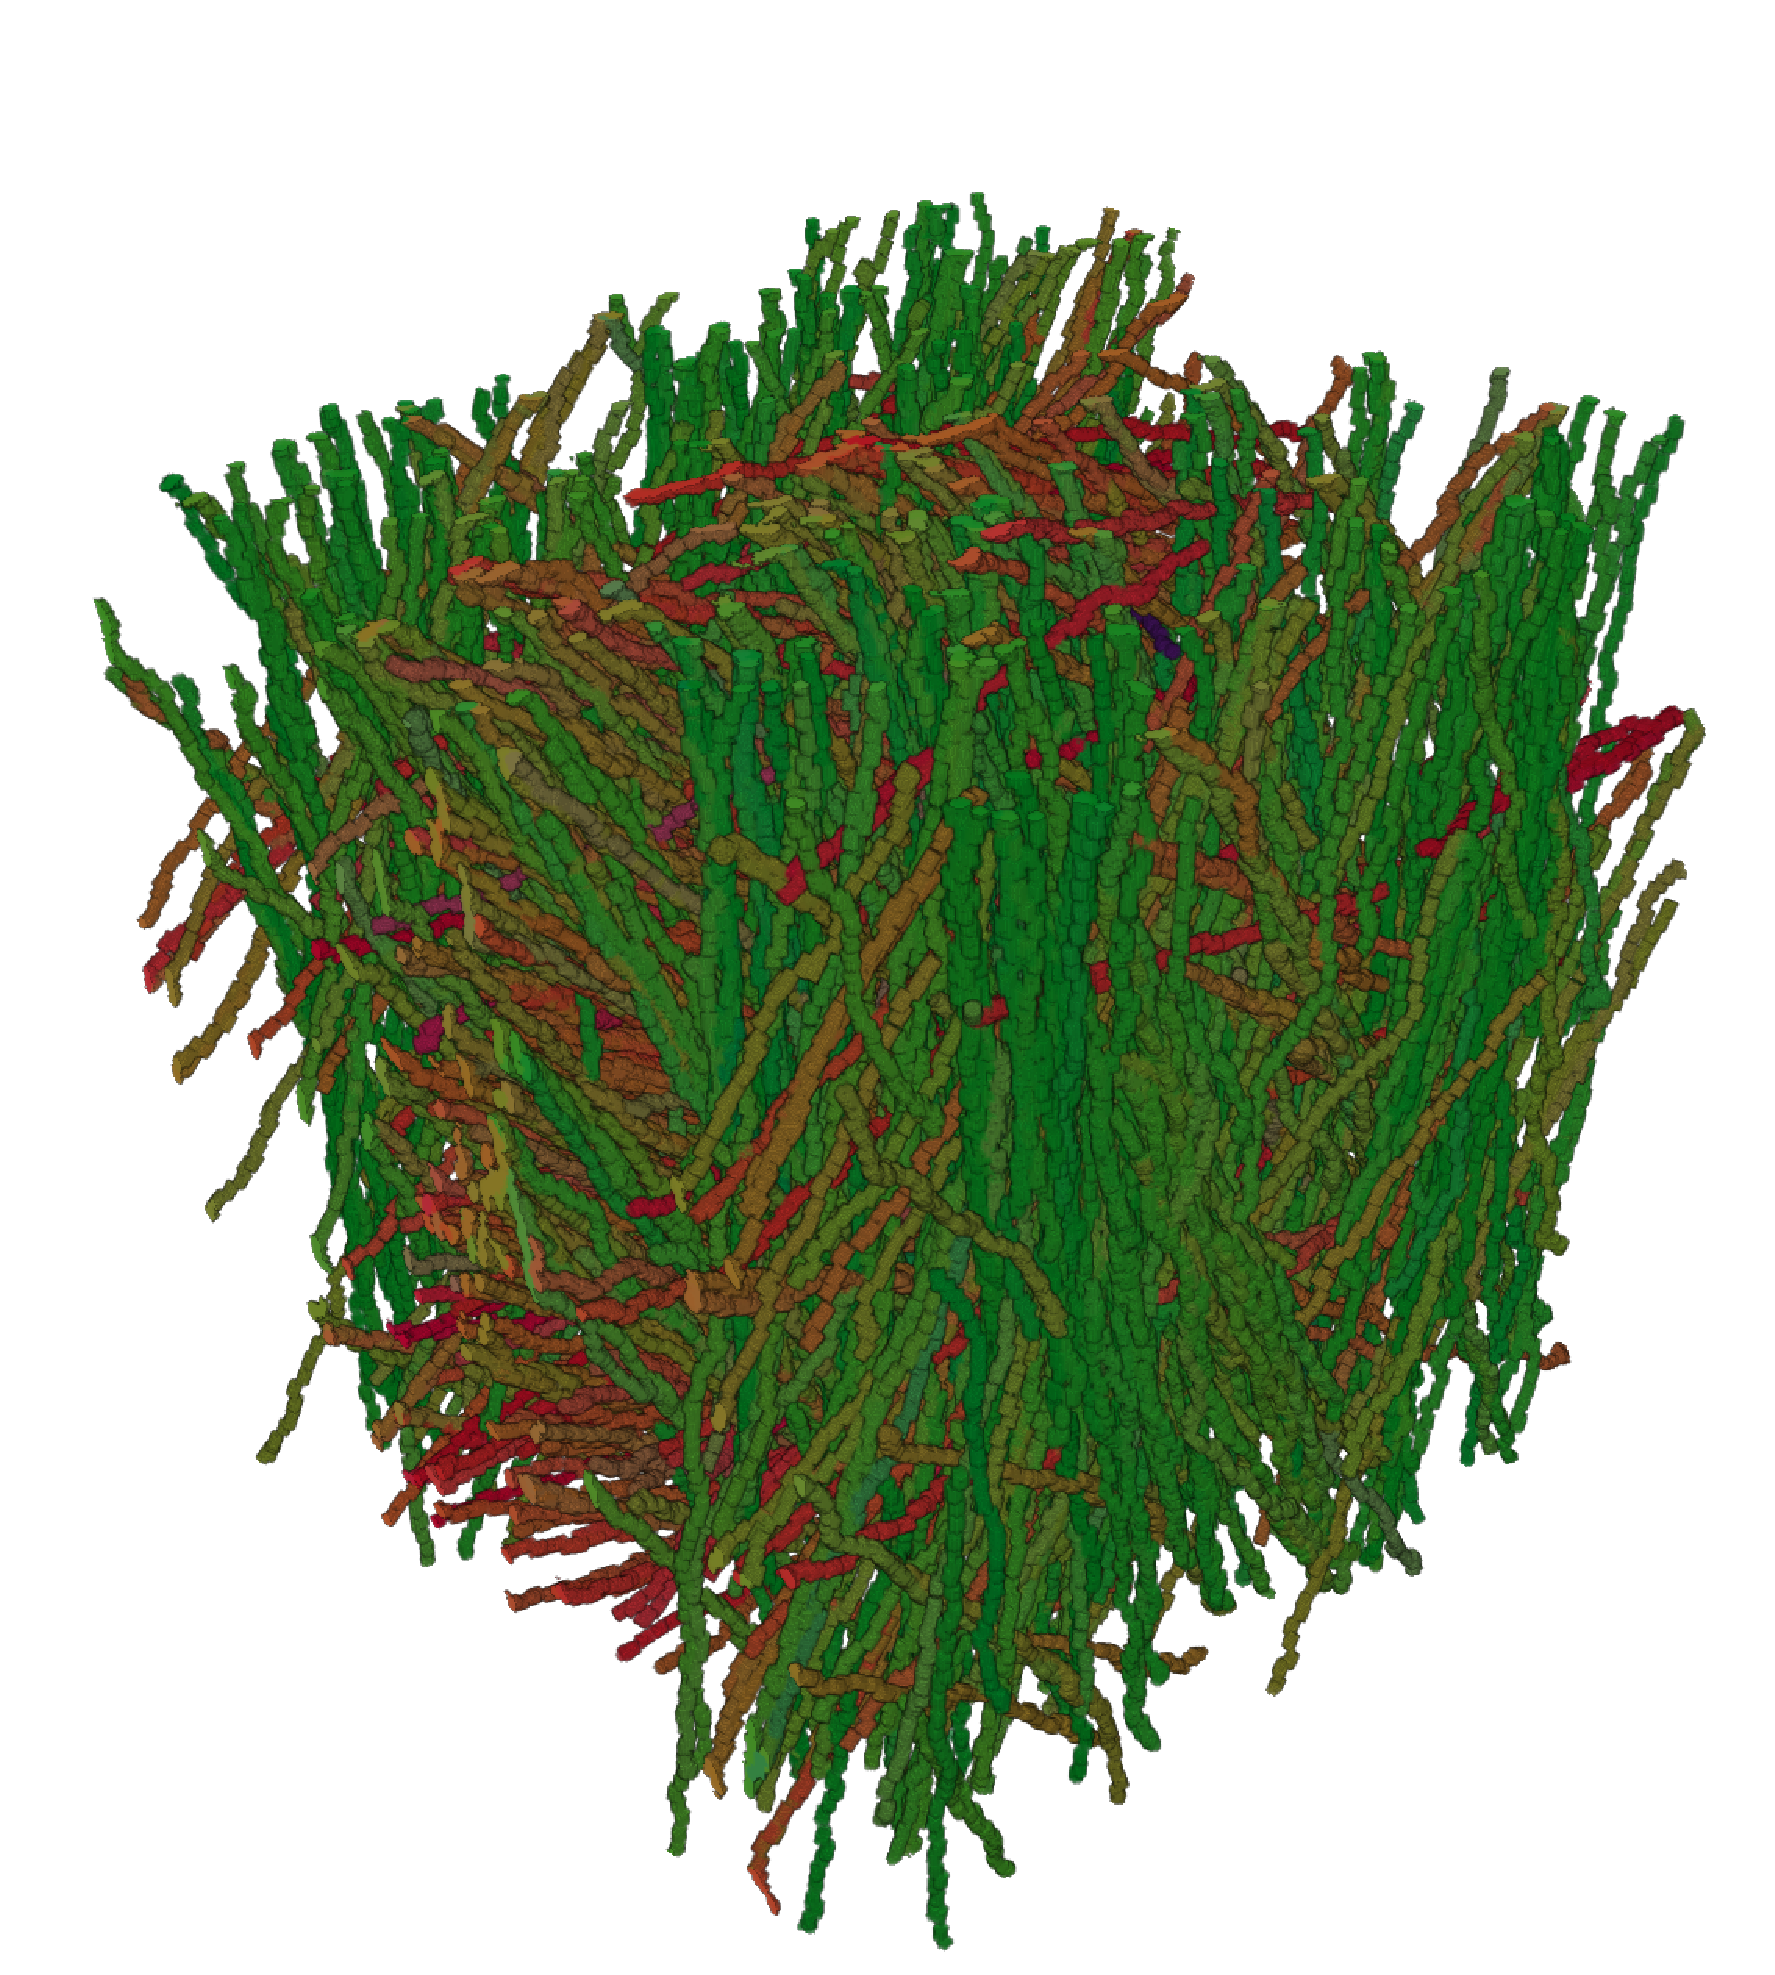
\includegraphics[width=0.25\linewidth]{imagesMT2014/glass-cluster-b.eps}}
  \subfloat[]{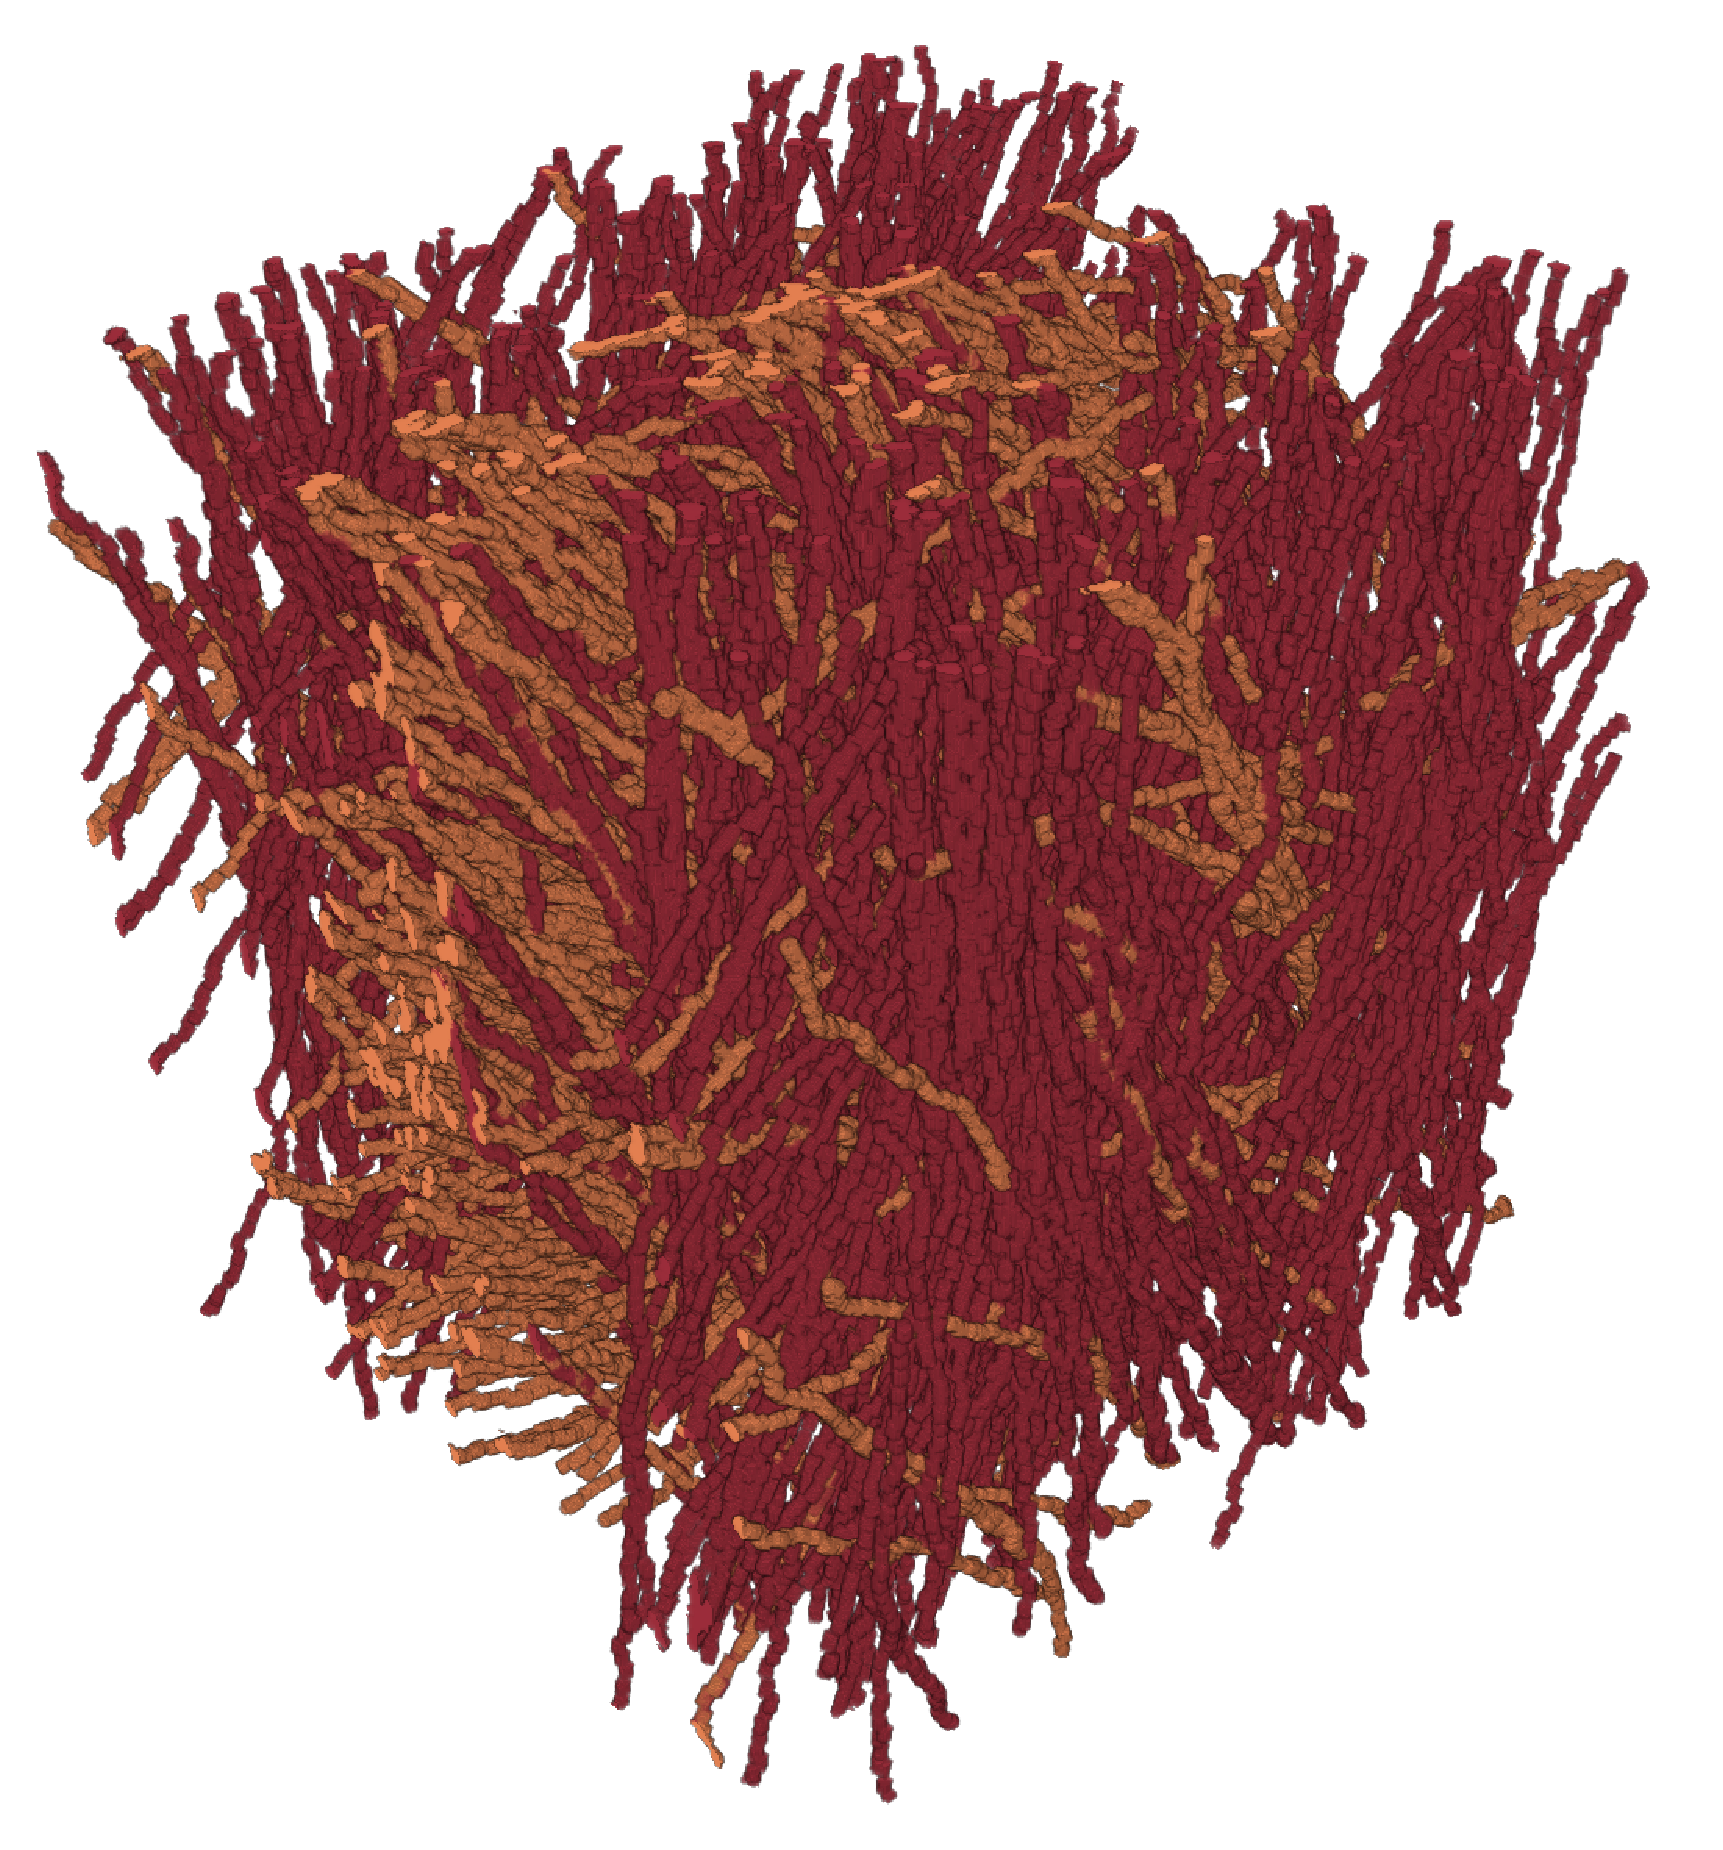
\includegraphics[width=0.25\linewidth]{imagesMT2014/glass-cluster-a.eps}}
  \caption{Our algorithm on a data set made of glass fibers. (a) The scalar dataset, (b) Depicts a slice from the data set, the  fibers are clearly demarcated from the rest of the matrix as oppose to the type of data  where it is hard to distinguish the fibers (Fig.~\ref{fig:data-char} or Fig.~\ref{fig:prepreg}A). (c) The result of the MetaTracts process, the colors are to help visualization. (d) The result of the orientation based clustering, the two clusters are marked red and yellow.}\label{fig:glass}
\end{figure}
\subsection{Glass Fibers}
\label{subsec:glass}
One simple way we used to validate the accuracy of shape and size of the extracted MetaTracts, is to run the MetaTract technique on Glass fibers.
Unlike the presented data, in glass the fibers are clearly visible (Fig.~\ref{fig:glass}(a)). We noted that the extracted MetaTracts closely followed the fibers in the data.
\subsection{Voxelization and surface extraction Extended}
\label{subsec:vox_ex}
The voxelization results and some of the meshes extracted from our second data set (Fig.~\ref{fig:prepreg}) are shown in Fig.~\ref{fig:vox_extended}.
\begin{figure}[h]
\centering
\subfloat[]{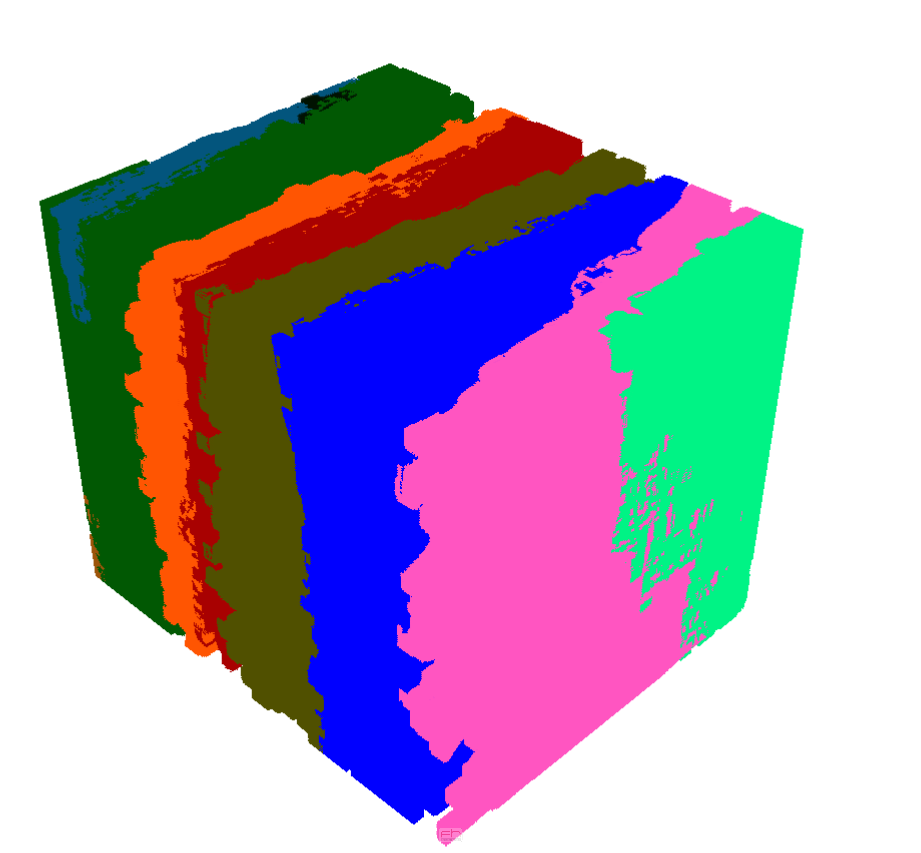
\includegraphics[width=0.2\textwidth]{imagesMT2014/crop-6-C2-vol}}
\subfloat[]{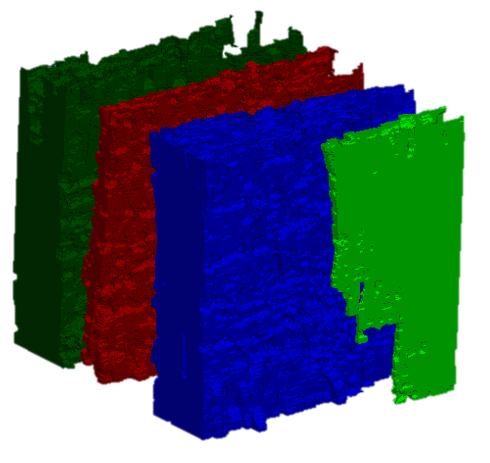
\includegraphics[width=0.2\textwidth]{imagesMT2014/mesh_prepreg_A}}
\\
\caption{(a) Voxelization of Fig.~\ref{fig:prepreg}C, (b) Shows some of the extracted meshes.}
\label{fig:vox_extended}
\end{figure}
\begin{figure}[h]
\centering
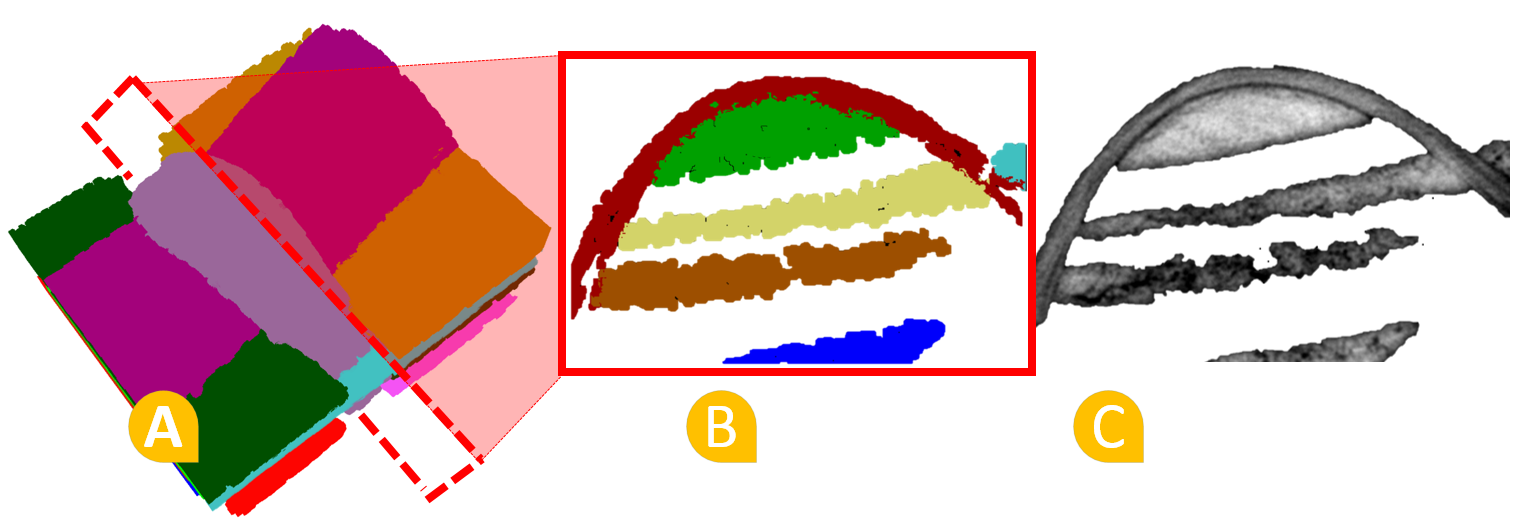
\includegraphics[width=0.5\textwidth]{imagesMT2014/UserStudy/vol_crop16}
\\
\caption{ A shows the Voxelization of Fig.~\ref{fig:data-char}. B shows a single slice. C the slice of original data. }
\label{fig:vox_extended_crop16}
\end{figure}

\begin{figure}[h]
\centering
\subfloat[]{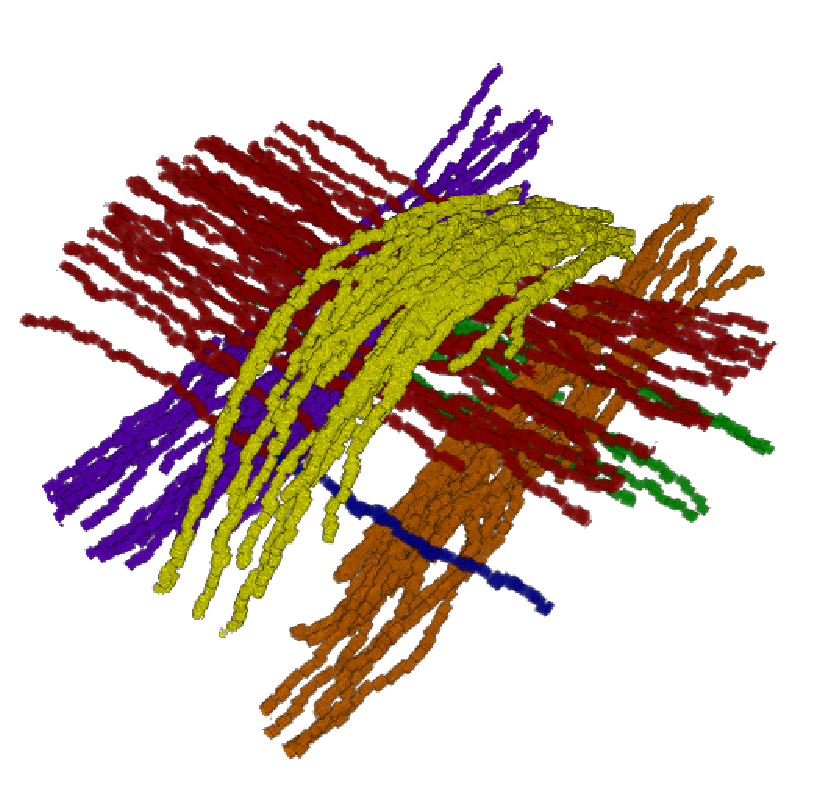
\includegraphics[width=0.25\linewidth]{imagesMT2014/compare-clus-1.eps}}
\subfloat[]{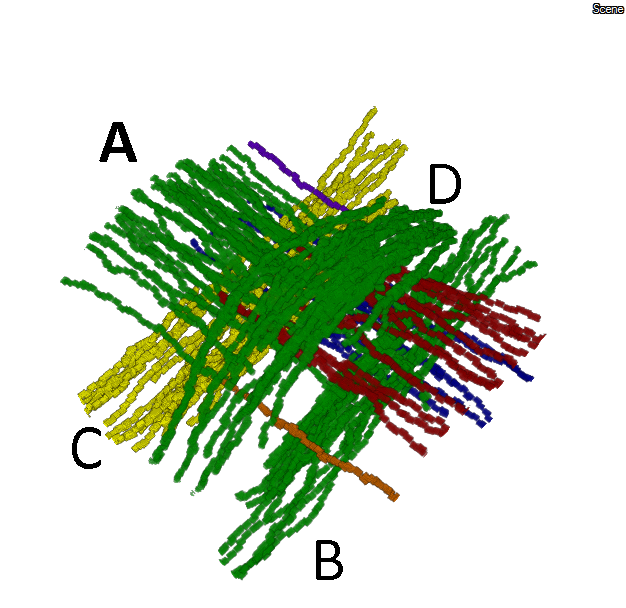
\includegraphics[width=0.33\linewidth]{imagesMT2014/compare-clus-3.png}}
\subfloat[]{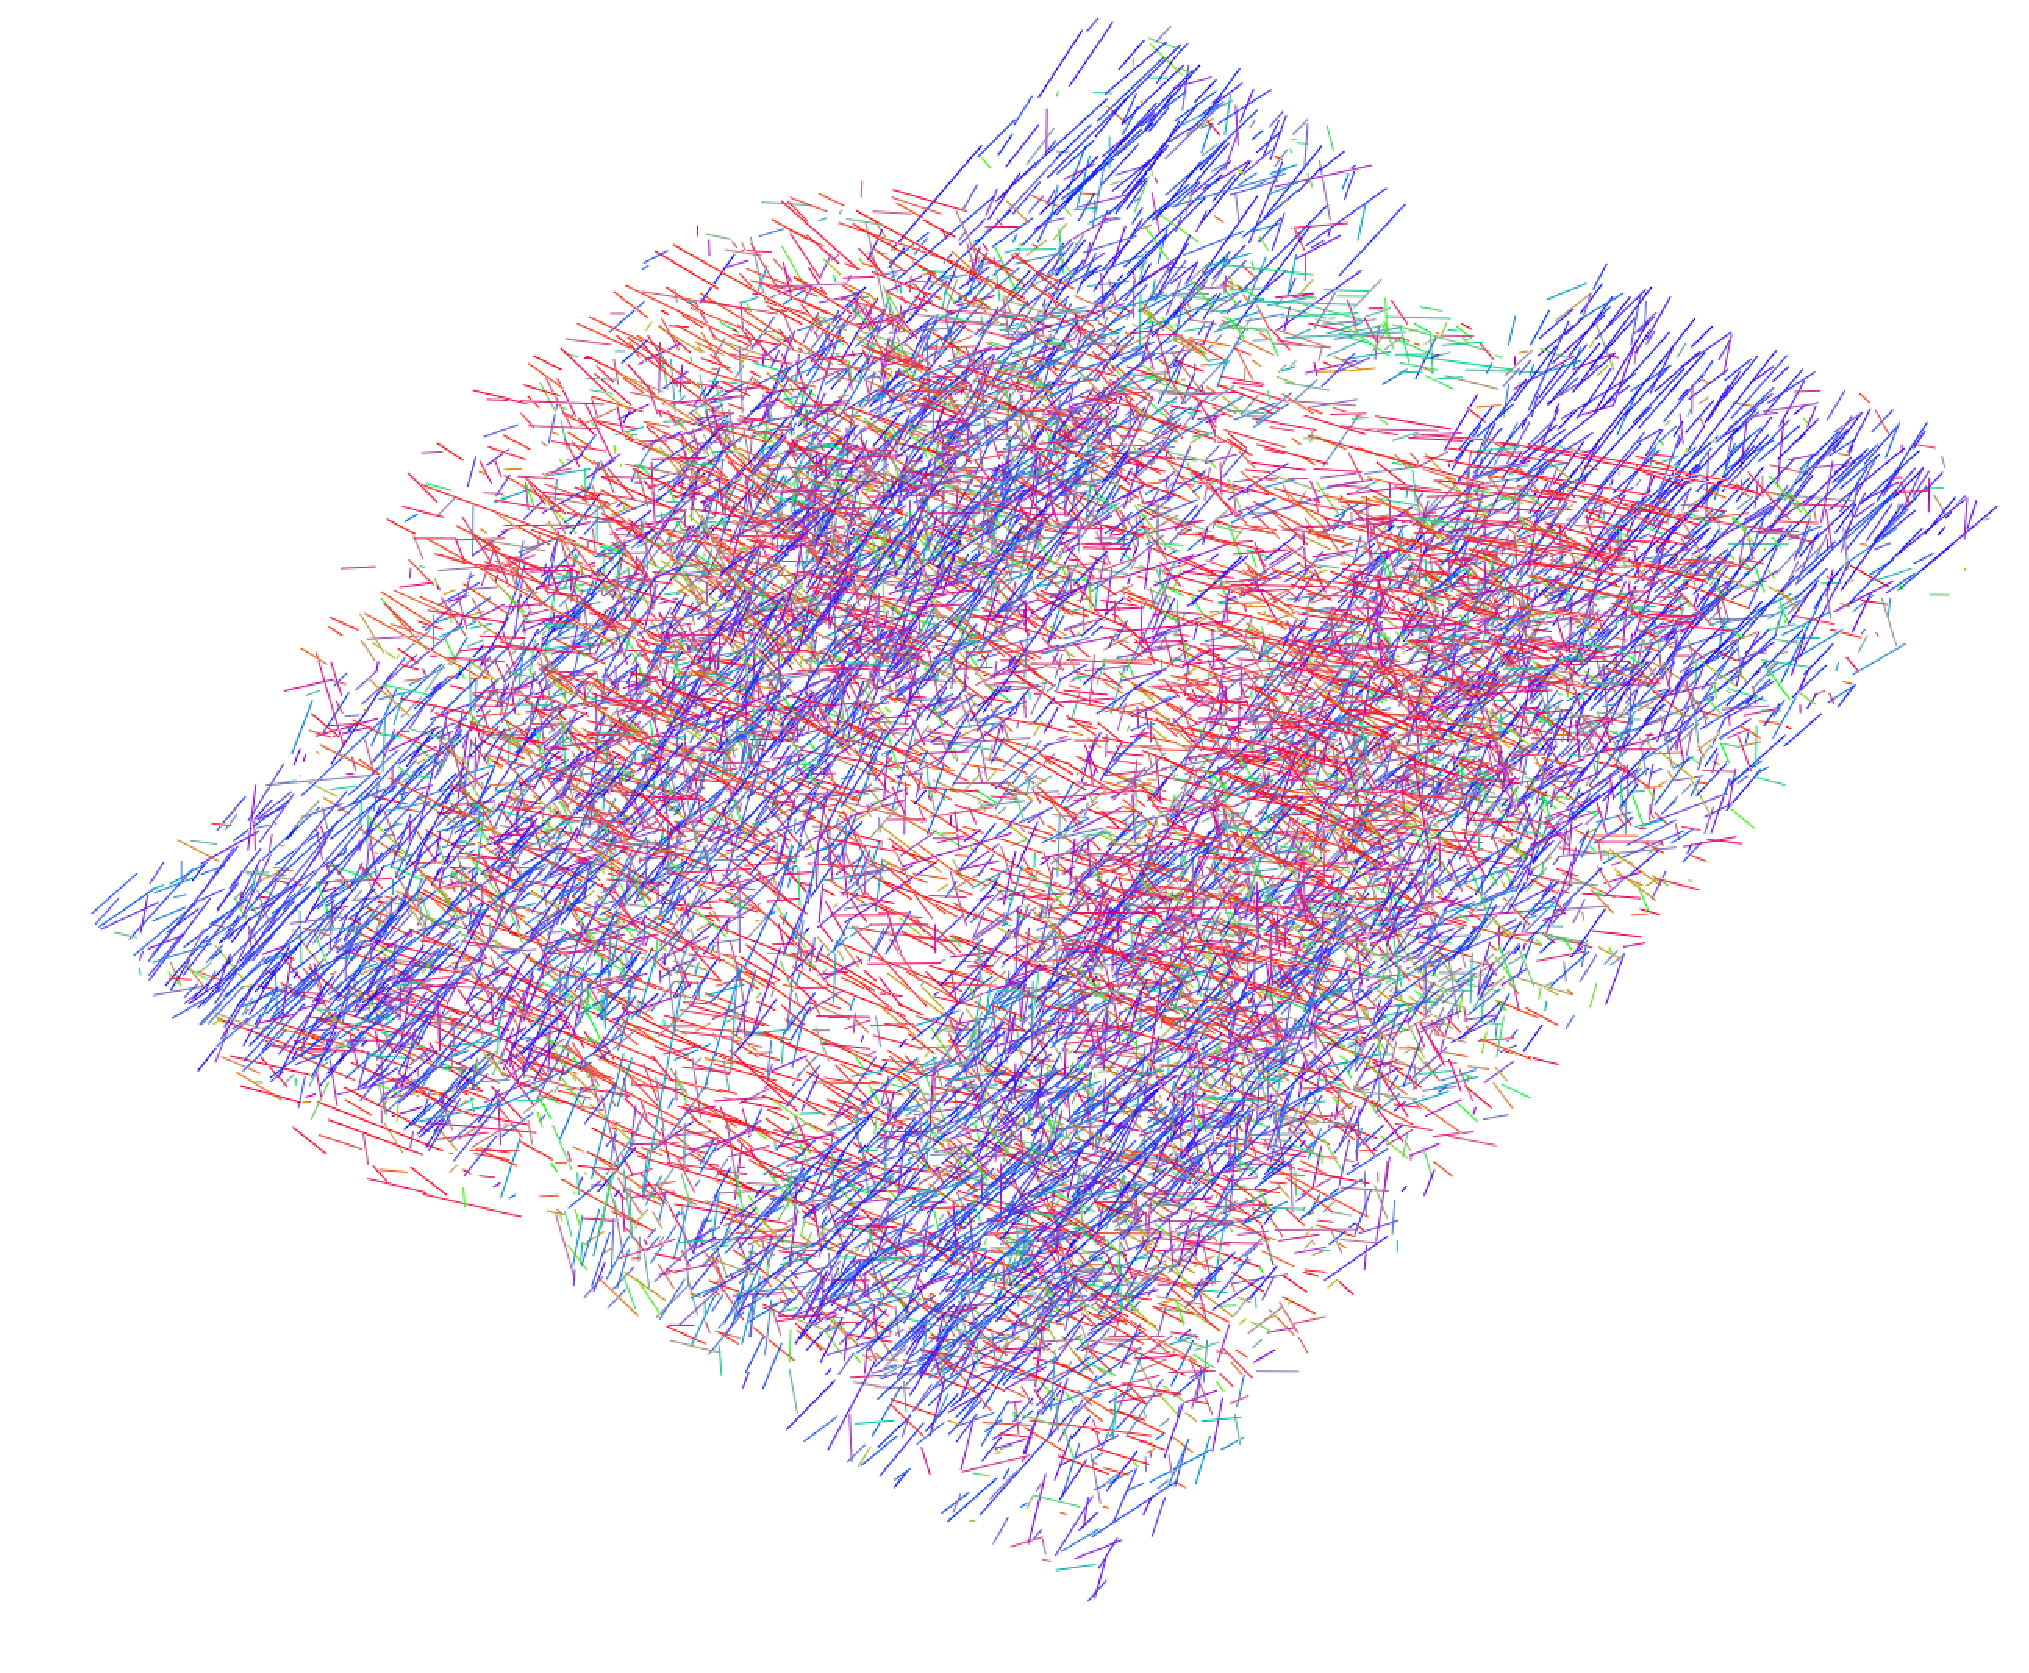
\includegraphics[width=0.25\linewidth]{imagesMT2014/Fiber_extraction_for_bundles_1.eps}}
\subfloat[]{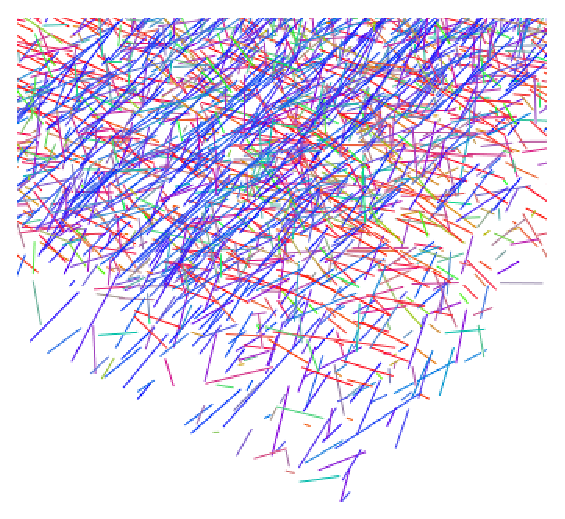
\includegraphics[width=0.25\linewidth]{imagesMT2014/Fiber_extraction_for_bundles_2.eps}}


   \caption{\textit{Comparison of clustering approaches}.(a)Our approach,  Orientation clustering into 2 classes followed by hierarchical clustering into 3 classes each. (b) Hierarchical clustering into 6 classes based on proximity alone.\\
   \textit{Comparison of fiber extraction approaches}. (c) Salaberger et al. ~\cite{Salaberger2011}, they generate numerous small length fibers and miss the curved bundles. (d) close up of the medial axis generated by their approach.}\label{fig:compare-3}
\end{figure}
\subsection {Comparison with hierarchical fiber clustering}
\label{subsec:compare}
Here we compare our framework against the single link clustering based on proximity alone as used by Zhang et al.\cite{Zhang2008}, Moberts et al.\cite{Moberts2005}. In Fig.~\ref{fig:compare-3}(a) we see the results of our approach. 169 fibers were first clustered based on orientation into 2 clusters and then each cluster was classified into 3 classes. In Fig.~\ref{fig:compare-3}(b) we see the results of direct hierarchical clustering of the distances into 6 classes. Direct hierarchical clustering based on proximity alone is not able to partition well, especially in the presence of partially overlapping tracts (Fig.~\ref{fig:length_distribution}(b)). Without the iterative approach (section~\ref{subsec:dist_clustering}) single linkage clustering tends to produce large clusters( `green' in Fig.~\ref{fig:compare-3}(b)) and outliers as separate cluster. The green cluster incorrectly contains MetaTracts from three different fiber bundles (A,D,B). In our approach all major fiber bundles are classified separately.
\subsection{Comparison with individual fiber extraction method}
 Recently  Salaberger et al.~\cite{Salaberger2011} provided a method to study the fiber length distribution in XCT data by extracting individual fibers. They employ the Hessian followed by a medial axis detection approach to follow  individual fibers. We apply their algorithm to show the short comings of applying current fiber detection approaches on our datasets. Fig.~\ref{fig:compare-3}(c-d) shows the comparison between our approaches. Fig.~\ref{fig:compare-3}(c) shows the medial axis extracted by their algorithm. Fig.~\ref{fig:compare-3}(d) shows a close up view. The width of the line is not important because cylinders could be drawn around (c) to produce the same effect as MetaTracts. Their ~\cite{Salaberger2011} approach is designed for well separated fibers, so in our data it produces numerous small length fibers, more over due to the high noise in the Hessians around the curved bundles and the lack of well separated fibers, their approach completely misses the curved bundle.
 
 
\subsection{Robustness to parameter changes}
\label{subsec:robustness}
Figure~\ref{fig:radius_3} shows the results of data set in Fig.~\ref{fig:data-char} clustered into 2 orientation cluster, and each orientation further clustered into 15 clusters (instead of 10 in Fig.~\ref{fig:len_dist_crop16}). Fig.~\ref{fig:radius_3}(a) shows the number of tracts, the median, minimum and maximum length of the MetaTracts in orientation cluster Fig.~\ref{fig:orientation_clustering}C.
The ground truth is 5 bundles. The radius of the individual MetaTract has been set to 3. We see that similar to Fig~\ref{fig:len_dist_crop16} the correct bundles are identified even with overestimated `h'. The median lengths of the extracted bundles are also similar. Fig~\ref{fig:radius_3}(c, d) shows the individual orientation bundles and Fig~\ref{fig:radius_3}(b) shows the combined bundles.
\begin{figure*}
\centering
\subfloat[]{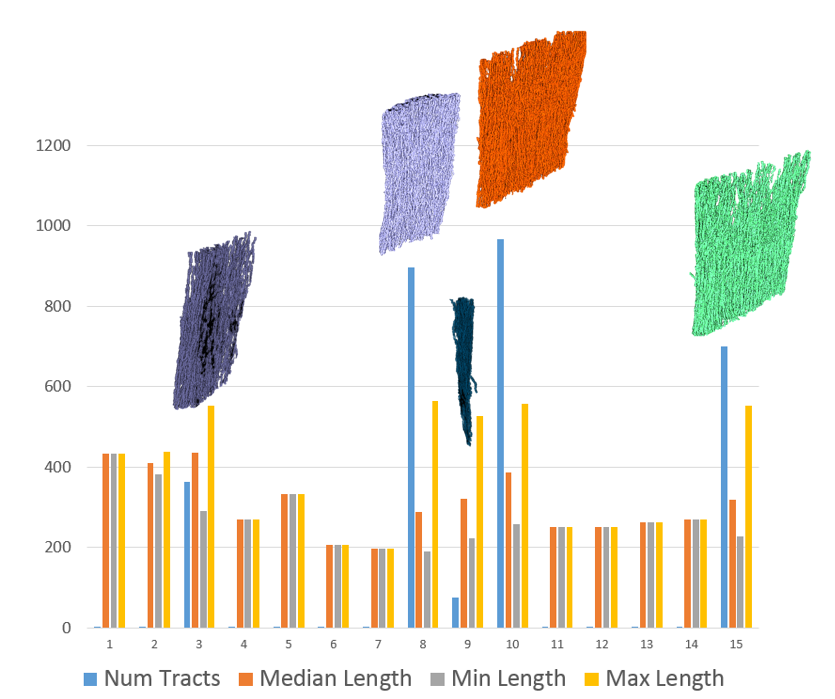
\includegraphics[width=0.6\textwidth]{imagesMT2014/Graph_crop16_3}}\\
\subfloat[]{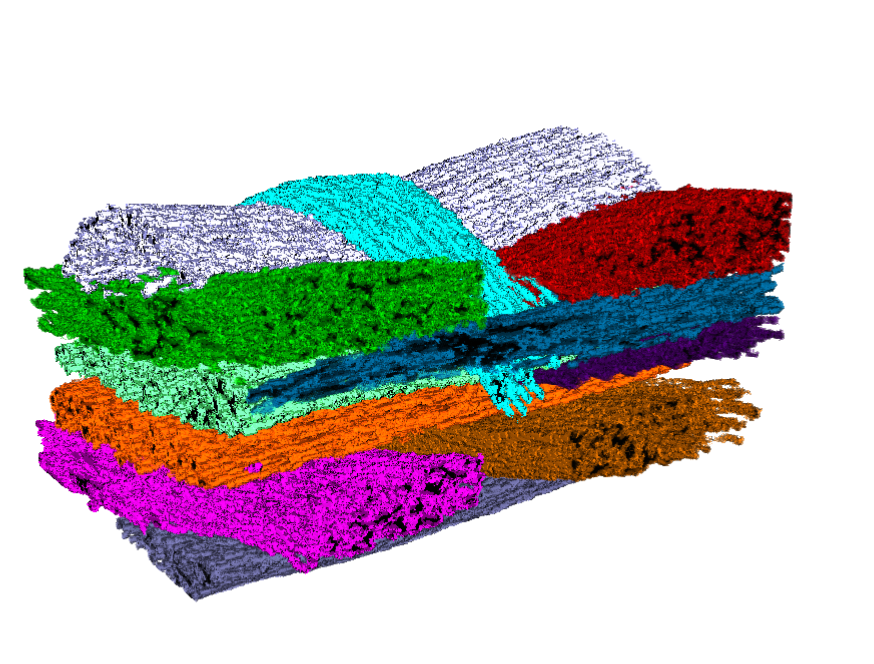
\includegraphics[width=0.3\textwidth]{imagesMT2014/crop-16/radius_3_orientC}}
\subfloat[]{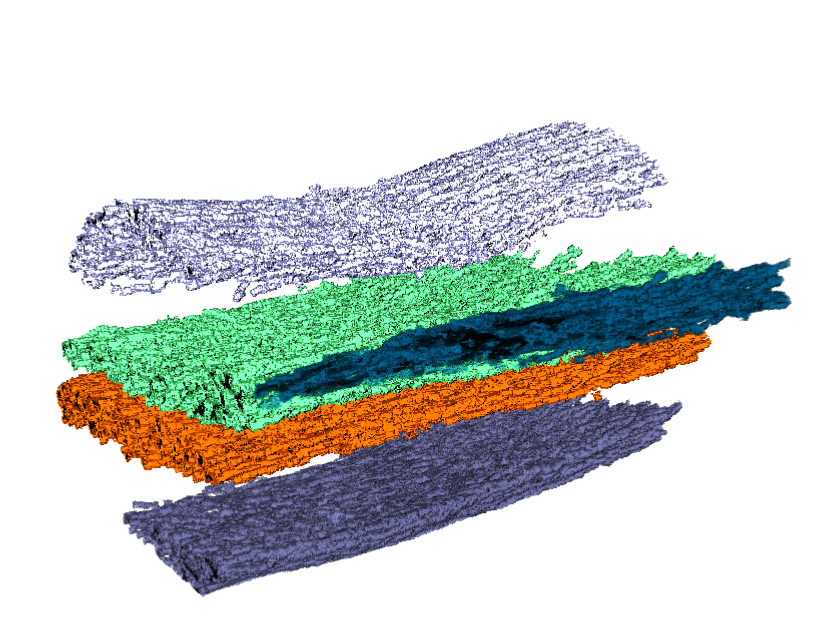
\includegraphics[width=0.25\textwidth]{imagesMT2014/crop-16/radius_3_orientA}}
\subfloat[]{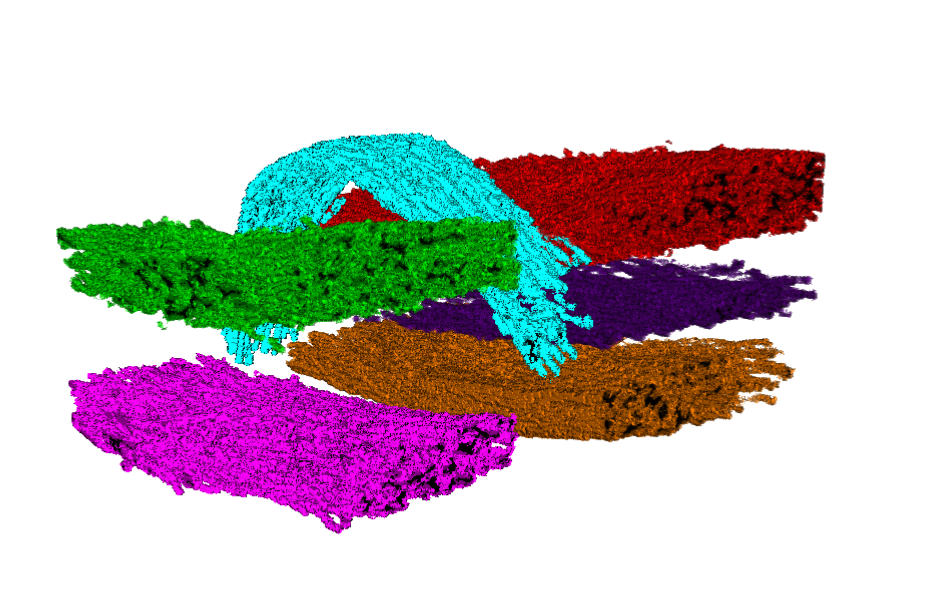
\includegraphics[width=0.25\textwidth]{imagesMT2014/crop-16/radius_3_orientB}}
\caption{(a) Number of tracts and median, minimum and maximum length of individual MetaTracts in the orientation cluster Fig.~\ref{fig:orientation_clustering}C, clustered into 15 clusters (Fig.~\ref{fig:crop-16-decomp}A top). The unit for length is the grid cube length.(b) shows the combined clusters from both the orientation, (c),(d) show the clustering of each orientation.}
\label{fig:radius_3}
\end{figure*}